\section{Exercise}

\begin{frame}{Scenario - WA WA WA WA WA ...}
\begin{center}
\only<1>{
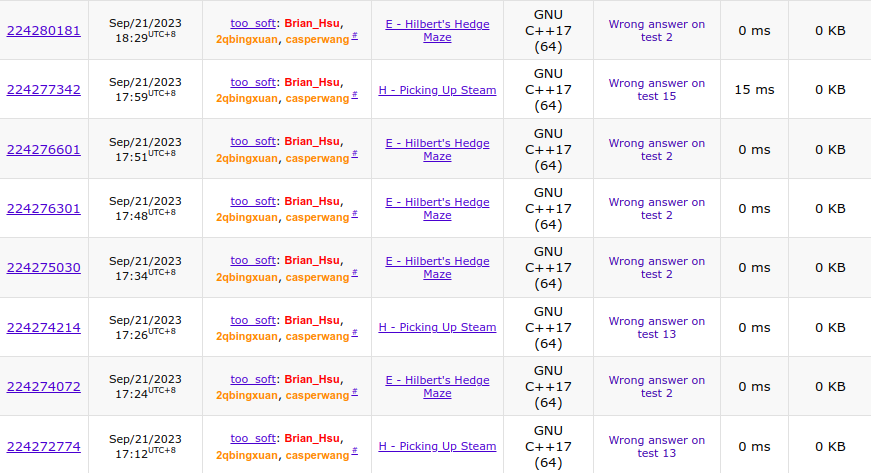
\includegraphics[width=12cm]{WA1.png}
}\only<2>{
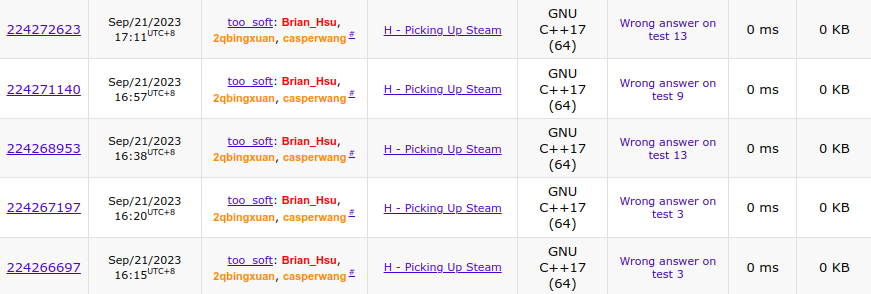
\includegraphics[width=12cm]{WA2.png}
}
\end{center}
\end{frame}

\begin{frame}{Scenario}
\begin{itemize}
\item The code with correct time complexity is complicated.
\item However, it is easy to write the code using brute force.
\end{itemize}
\end{frame}

\begin{frame}{How to Debug}
\begin{itemize}
\item The WA test case might help.
\item The judge does not show the WA test case.
\item Generate it yourself.
\item Compare with the output of your brute force code.
\end{itemize}
\end{frame}

\begin{frame}{Generator}
\begin{itemize}
\item Randomly generate some tests in the given range.
\item Example generator \t{gen.c} of \href{https://judgegirl.csie.org/problem/0/3}{Print Two Numbers}.
\lstinputlisting[language=c]{exercise/gen.c}
\item Compile \t{gen.c} to \t{gen}, and run \t{./gen arg}.
\item The output is determined by the argument \t{arg}.
\end{itemize}
\end{frame}

\begin{frame}{Brute Force Solution}
\begin{itemize}
\item A code that generates the correct output.
\item Example brute force solution \t{sol.c} of \href{https://judgegirl.csie.org/problem/0/3}{Print Two Numbers}.
\lstinputlisting[language=c]{exercise/sol.c}
\end{itemize}
\end{frame}

\begin{frame}{The WA Code}
\begin{itemize}
\item The code that got WA on the judge.
\item Example WA code \t{wa.c} of \href{https://judgegirl.csie.org/problem/0/3}{Print Two Numbers}.
\lstinputlisting[language=c]{exercise/wa.c}
\end{itemize}
\end{frame}

\begin{frame}{Debugger}
\begin{itemize}
\only<1>{
\item Write a shell script (called \t{debugger.sh}).
\item Usage: \t{./debugger.sh <Generator> <Code 1> <Code 2> <time>}
\item The shell script should do the following things:
\begin{itemize}
\item Compile \t{<Generator>}, \t{<Code 1>}, \t{<Code 2>} into \t{gen}, \t{a}, \t{b}, respectively.
\item For \t{i=1} to \t{<time>}, use the output generated by \t{./gen i} as the input \t{in.txt} of \t{a} and \t{b}.
\item If the outputs of running \t{a} and \t{b} are different, then output the debug message (the format is in the next page), and then \t{debugger.sh} should exit.
\end{itemize}
}\only<2>{
\item Output format:
\begin{itemize}
\item First line: \t{Test \$i:}
\item Second line: \t{Input:}
\item Print the content of \t{in.txt} with $20$ '-' each above and below.
\item Next line: \t{Output of <Code 1>:}
\item Print the output of running \t{a} with $20$ '-' each above and below.
\item Next line: \t{Output of <Code 2>:}
\item Print the output of running \t{b} with $20$ '-' each above and below.
\end{itemize}
}\only<3>{
\item Example output of \t{./debugger.sh gen.c sol.c wa.c 10}:
\lstinputlisting{exercise/output}
}
\end{itemize}
\end{frame}

\begin{frame}{Time Limit}
\begin{itemize}
\item Time limit: $1$ minute.
\item \t{<time>}$\leq1000$.
\item If \t{<Code A>}, \t{<Code B>} are guaranteed to finish running in $s$ seconds, then $s\times$\t{<time>}$\leq50$ is guaranteed.
\end{itemize}
\end{frame}

\begin{frame}{Submission}
\begin{itemize}
\item Deadline: 2024/2/29 23:59
\item Submit your code \href{https://forms.gle/ruzJYMdvkmZ6u9CY9}{here}.
\item Check your result \href{https://docs.google.com/spreadsheets/d/1WM8s-83BM6E4rtIQqPEAteCGHQWJ7LZSKluali3owi0/edit?usp=sharing}{here}.
\item Use base64 to encode a file: \t{base64 FILE}
\item Calculate the sha1sum of a file: \t{sha1sum FILE}
\item $0$ point for plagiarism.
\item $0$ point for any malicious behavior in your script.
\item Your script should NOT create nor remove things that are not in the current working directory.
\item Your script will be run on the workstation.
\end{itemize}
\end{frame}

\begin{frame}{Hints}
\begin{itemize}
\item {[}02/27 11:04{]}: Notice the output of the following code:
\lstinputlisting[language=bash]{eatnewline.sh}
\end{itemize}
\end{frame}
